\documentclass{standalone}
\usepackage{tikz}
\usetikzlibrary{patterns, positioning}


\begin{document}
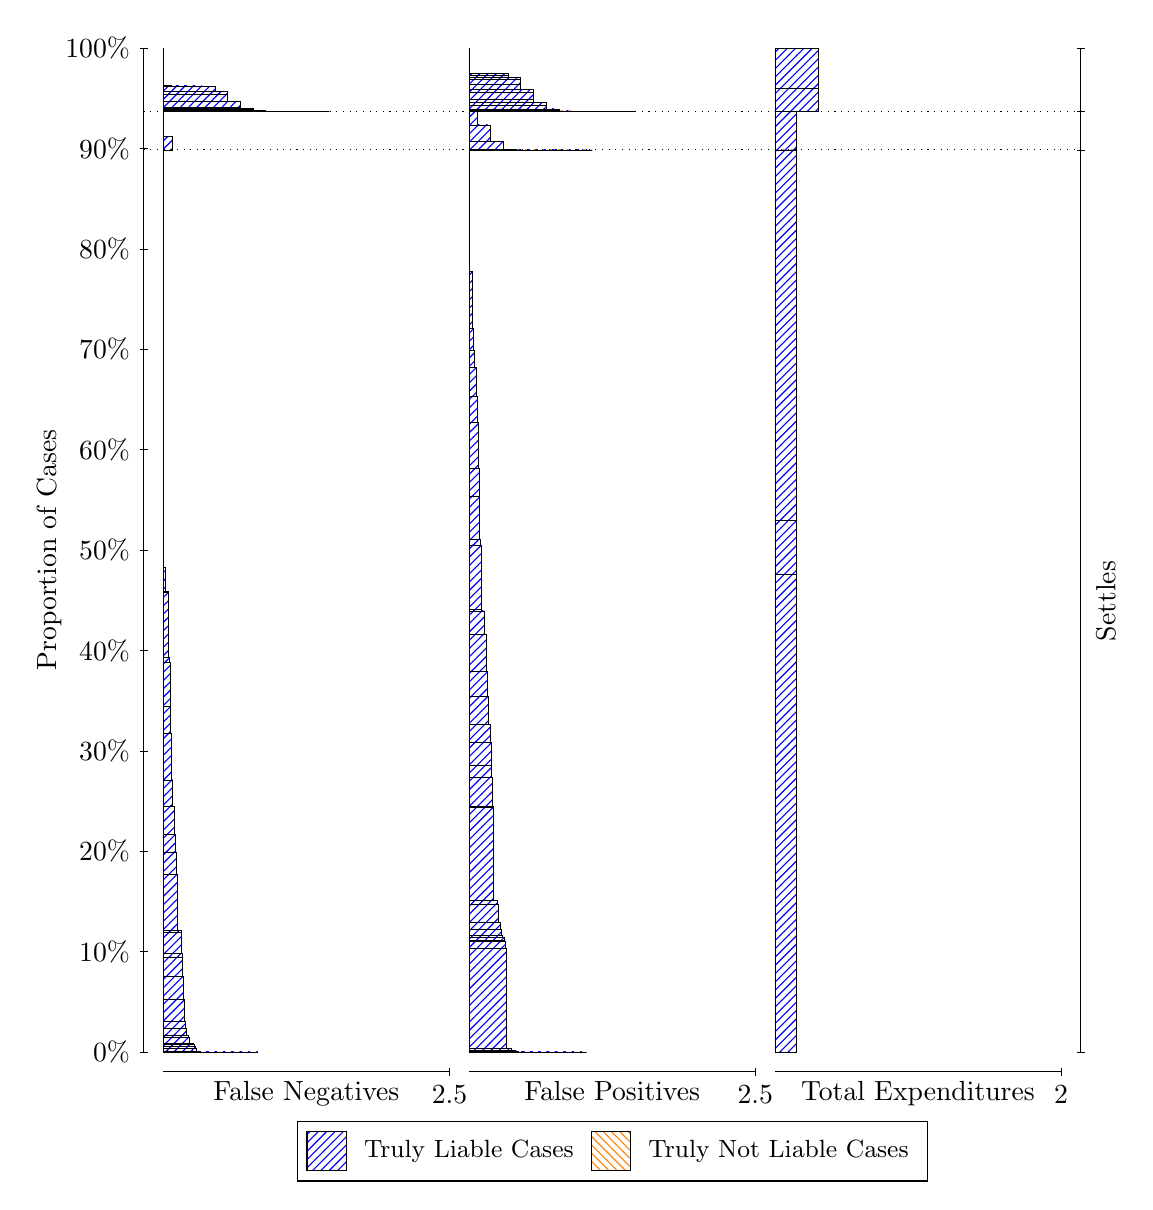
\begin{tikzpicture}
\draw[black, very thin] (1.5,1.75) -- (1.5,14.5);
\node[rotate=90, text=black, anchor=center] at (0.3, 8.125) {Proportion of Cases};
\draw[black, very thin] (1.45,1.75) -- (1.55,1.75);
\node[text=black, anchor=east] at (1.45, 1.75) {0\%};
\draw[black, very thin] (1.45,3.025) -- (1.55,3.025);
\node[text=black, anchor=east] at (1.45, 3.025) {10\%};
\draw[black, very thin] (1.45,4.3) -- (1.55,4.3);
\node[text=black, anchor=east] at (1.45, 4.3) {20\%};
\draw[black, very thin] (1.45,5.575) -- (1.55,5.575);
\node[text=black, anchor=east] at (1.45, 5.575) {30\%};
\draw[black, very thin] (1.45,6.85) -- (1.55,6.85);
\node[text=black, anchor=east] at (1.45, 6.85) {40\%};
\draw[black, very thin] (1.45,8.125) -- (1.55,8.125);
\node[text=black, anchor=east] at (1.45, 8.125) {50\%};
\draw[black, very thin] (1.45,9.4) -- (1.55,9.4);
\node[text=black, anchor=east] at (1.45, 9.4) {60\%};
\draw[black, very thin] (1.45,10.675) -- (1.55,10.675);
\node[text=black, anchor=east] at (1.45, 10.675) {70\%};
\draw[black, very thin] (1.45,11.95) -- (1.55,11.95);
\node[text=black, anchor=east] at (1.45, 11.95) {80\%};
\draw[black, very thin] (1.45,13.225) -- (1.55,13.225);
\node[text=black, anchor=east] at (1.45, 13.225) {90\%};
\draw[black, very thin] (1.45,14.5) -- (1.55,14.5);
\node[text=black, anchor=east] at (1.45, 14.5) {100\%};

\draw[black, very thin] (13.4,1.75) -- (13.4,14.5);
\draw[black, very thin] (13.35,1.75) -- (13.45,1.75);
\node[anchor=west] at (13.35, 1.75) {};
\draw[black, very thin] (13.35,13.206) -- (13.45,13.206);
\node[anchor=west] at (13.35, 13.206) {};
\draw[black, very thin] (13.35,13.699) -- (13.45,13.699);
\node[anchor=west] at (13.35, 13.699) {};
\draw[black, very thin] (13.35,14.5) -- (13.45,14.5);
\node[anchor=west] at (13.35, 14.5) {};

\draw[black, very thin, pattern color=blue, pattern=north east lines] (1.75,1.75) rectangle (2.949,1.75);
\draw[black, very thin, pattern color=blue, pattern=north east lines] (1.75,1.75) rectangle (2.8037,1.75);
\draw[black, very thin, pattern color=blue, pattern=north east lines] (1.75,1.75) rectangle (2.7875,1.75);
\draw[black, very thin, pattern color=blue, pattern=north east lines] (1.75,1.75) rectangle (2.6583,1.75);
\draw[black, very thin, pattern color=blue, pattern=north east lines] (1.75,1.75) rectangle (2.6422,1.75);
\draw[black, very thin, pattern color=blue, pattern=north east lines] (1.75,1.75) rectangle (2.626,1.75);
\draw[black, very thin, pattern color=blue, pattern=north east lines] (1.75,1.75) rectangle (2.513,1.75);
\draw[black, very thin, pattern color=blue, pattern=north east lines] (1.75,1.75) rectangle (2.4969,1.75);
\draw[black, very thin, pattern color=blue, pattern=north east lines] (1.75,1.75) rectangle (2.4807,1.75);
\draw[black, very thin, pattern color=blue, pattern=north east lines] (1.75,1.75) rectangle (2.4646,1.75);
\draw[black, very thin, pattern color=blue, pattern=north east lines] (1.75,1.75) rectangle (2.4403,1.75);
\draw[black, very thin, pattern color=blue, pattern=north east lines] (1.75,1.75) rectangle (2.3677,1.7501);
\draw[black, very thin, pattern color=blue, pattern=north east lines] (1.75,1.7501) rectangle (2.3515,1.7502);
\draw[black, very thin, pattern color=blue, pattern=north east lines] (1.75,1.7502) rectangle (2.3354,1.7507);
\draw[black, very thin, pattern color=blue, pattern=north east lines] (1.75,1.7507) rectangle (2.3192,1.7512);
\draw[black, very thin, pattern color=blue, pattern=north east lines] (1.75,1.7512) rectangle (2.3031,1.7518);
\draw[black, very thin, pattern color=blue, pattern=north east lines] (1.75,1.7518) rectangle (2.295,1.7521);
\draw[black, very thin, pattern color=blue, pattern=north east lines] (1.75,1.7521) rectangle (2.2789,1.7521);
\draw[black, very thin, pattern color=blue, pattern=north east lines] (1.75,1.7521) rectangle (2.2223,1.7543);
\draw[black, very thin, pattern color=blue, pattern=north east lines] (1.75,1.7543) rectangle (2.2062,1.7587);
\draw[black, very thin, pattern color=blue, pattern=north east lines] (1.75,1.7587) rectangle (2.19,1.7641);
\draw[black, very thin, pattern color=blue, pattern=north east lines] (1.75,1.7641) rectangle (2.1739,1.7917);
\draw[black, very thin, pattern color=blue, pattern=north east lines] (1.75,1.7917) rectangle (2.1577,1.8174);
\draw[black, very thin, pattern color=blue, pattern=north east lines] (1.75,1.8174) rectangle (2.1497,1.8262);
\draw[black, very thin, pattern color=blue, pattern=north east lines] (1.75,1.8262) rectangle (2.1416,1.8525);
\draw[black, very thin, pattern color=blue, pattern=north east lines] (1.75,1.8525) rectangle (2.1335,1.8571);
\draw[black, very thin, pattern color=blue, pattern=north east lines] (1.75,1.8571) rectangle (2.1174,1.8572);
\draw[black, very thin, pattern color=blue, pattern=north east lines] (1.75,1.8572) rectangle (2.077,1.9313);
\draw[black, very thin, pattern color=blue, pattern=north east lines] (1.75,1.9313) rectangle (2.0609,1.9684);
\draw[black, very thin, pattern color=blue, pattern=north east lines] (1.75,1.9684) rectangle (2.0447,2.0473);
\draw[black, very thin, pattern color=blue, pattern=north east lines] (1.75,2.0473) rectangle (2.0286,2.1456);
\draw[black, very thin, pattern color=blue, pattern=north east lines] (1.75,2.1456) rectangle (2.0124,2.419);
\draw[black, very thin, pattern color=blue, pattern=north east lines] (1.75,2.419) rectangle (2.0043,2.7118);
\draw[black, very thin, pattern color=blue, pattern=north east lines] (1.75,2.7118) rectangle (1.9963,2.9575);
\draw[black, very thin, pattern color=blue, pattern=north east lines] (1.75,2.9575) rectangle (1.9882,3.0027);
\draw[black, very thin, pattern color=blue, pattern=north east lines] (1.75,3.0027) rectangle (1.9801,3.2745);
\draw[black, very thin, pattern color=blue, pattern=north east lines] (1.75,3.2745) rectangle (1.972,3.2942);
\draw[black, very thin, pattern color=blue, pattern=north east lines] (1.75,3.2942) rectangle (1.9559,3.2946);
\draw[black, very thin, pattern color=blue, pattern=north east lines] (1.75,3.2946) rectangle (1.9317,4.0097);
\draw[black, very thin, pattern color=blue, pattern=north east lines] (1.75,4.0097) rectangle (1.9155,4.292);
\draw[black, very thin, pattern color=blue, pattern=north east lines] (1.75,4.292) rectangle (1.8994,4.5097);
\draw[black, very thin, pattern color=blue, pattern=north east lines] (1.75,4.5097) rectangle (1.8832,4.8758);
\draw[black, very thin, pattern color=blue, pattern=north east lines] (1.75,4.8758) rectangle (1.8671,5.2067);
\draw[black, very thin, pattern color=blue, pattern=north east lines] (1.75,5.2067) rectangle (1.8509,5.7992);
\draw[black, very thin, pattern color=blue, pattern=north east lines] (1.75,5.7992) rectangle (1.8429,6.1428);
\draw[black, very thin, pattern color=blue, pattern=north east lines] (1.75,6.1428) rectangle (1.8348,6.6935);
\draw[black, very thin, pattern color=blue, pattern=north east lines] (1.75,6.6935) rectangle (1.8267,6.7651);
\draw[black, very thin, pattern color=blue, pattern=north east lines] (1.75,6.7651) rectangle (1.8186,7.5851);
\draw[black, very thin, pattern color=blue, pattern=north east lines] (1.75,7.5851) rectangle (1.8106,7.6037);
\draw[black, very thin, pattern color=blue, pattern=north east lines] (1.75,7.6037) rectangle (1.7944,7.6041);
\draw[black, very thin, pattern color=blue, pattern=north east lines] (1.75,7.6041) rectangle (1.7702,7.9061);
\draw[black, very thin, pattern color=blue, pattern=north east lines] (1.75,7.9061) rectangle (1.754,8.3758);
\draw[black, very thin, pattern color=orange, pattern=north west lines] (1.75,8.3758) rectangle (1.75,8.3758);
\draw[black, very thin, pattern color=blue, pattern=north east lines] (1.75,8.3758) rectangle (1.75,13.206);
\draw[black, very thin, pattern color=blue, pattern=north east lines] (1.75,13.206) rectangle (1.859,13.379);
\draw[black, very thin, pattern color=orange, pattern=north west lines] (1.75,13.379) rectangle (1.75,13.379);
\draw[black, very thin, pattern color=blue, pattern=north east lines] (1.75,13.379) rectangle (1.75,13.699);
\draw[black, very thin, pattern color=blue, pattern=north east lines] (1.75,13.699) rectangle (3.8573,13.699);
\draw[black, very thin, pattern color=blue, pattern=north east lines] (1.75,13.699) rectangle (3.6959,13.699);
\draw[black, very thin, pattern color=blue, pattern=north east lines] (1.75,13.699) rectangle (3.5344,13.699);
\draw[black, very thin, pattern color=blue, pattern=north east lines] (1.75,13.699) rectangle (3.5344,13.699);
\draw[black, very thin, pattern color=blue, pattern=north east lines] (1.75,13.699) rectangle (3.3729,13.699);
\draw[black, very thin, pattern color=blue, pattern=north east lines] (1.75,13.699) rectangle (3.2114,13.699);
\draw[black, very thin, pattern color=blue, pattern=north east lines] (1.75,13.699) rectangle (3.0499,13.705);
\draw[black, very thin, pattern color=blue, pattern=north east lines] (1.75,13.705) rectangle (2.8884,13.716);
\draw[black, very thin, pattern color=blue, pattern=north east lines] (1.75,13.716) rectangle (2.8884,13.733);
\draw[black, very thin, pattern color=blue, pattern=north east lines] (1.75,13.733) rectangle (2.727,13.75);
\draw[black, very thin, pattern color=blue, pattern=north east lines] (1.75,13.75) rectangle (2.727,13.821);
\draw[black, very thin, pattern color=blue, pattern=north east lines] (1.75,13.821) rectangle (2.5655,13.918);
\draw[black, very thin, pattern color=blue, pattern=north east lines] (1.75,13.918) rectangle (2.5655,13.951);
\draw[black, very thin, pattern color=blue, pattern=north east lines] (1.75,13.951) rectangle (2.5009,13.951);
\draw[black, very thin, pattern color=blue, pattern=north east lines] (1.75,13.951) rectangle (2.404,14.012);
\draw[black, very thin, pattern color=blue, pattern=north east lines] (1.75,14.012) rectangle (2.3394,14.012);
\draw[black, very thin, pattern color=blue, pattern=north east lines] (1.75,14.012) rectangle (2.2425,14.012);
\draw[black, very thin, pattern color=blue, pattern=north east lines] (1.75,14.012) rectangle (2.2425,14.016);
\draw[black, very thin, pattern color=blue, pattern=north east lines] (1.75,14.016) rectangle (2.2425,14.019);
\draw[black, very thin, pattern color=blue, pattern=north east lines] (1.75,14.019) rectangle (2.1779,14.019);
\draw[black, very thin, pattern color=blue, pattern=north east lines] (1.75,14.019) rectangle (2.1779,14.019);
\draw[black, very thin, pattern color=blue, pattern=north east lines] (1.75,14.019) rectangle (2.081,14.019);
\draw[black, very thin, pattern color=blue, pattern=north east lines] (1.75,14.019) rectangle (2.081,14.019);
\draw[black, very thin, pattern color=blue, pattern=north east lines] (1.75,14.019) rectangle (2.0164,14.02);
\draw[black, very thin, pattern color=blue, pattern=north east lines] (1.75,14.02) rectangle (2.0164,14.02);
\draw[black, very thin, pattern color=blue, pattern=north east lines] (1.75,14.02) rectangle (1.9196,14.02);
\draw[black, very thin, pattern color=blue, pattern=north east lines] (1.75,14.02) rectangle (1.9196,14.02);
\draw[black, very thin, pattern color=blue, pattern=north east lines] (1.75,14.02) rectangle (1.855,14.02);
\draw[black, very thin, pattern color=blue, pattern=north east lines] (1.75,14.02) rectangle (1.855,14.022);
\draw[black, very thin, pattern color=blue, pattern=north east lines] (1.75,14.022) rectangle (1.7581,14.022);
\draw[black, very thin, pattern color=blue, pattern=north east lines] (1.75,14.022) rectangle (1.7581,14.022);
\draw[black, very thin, pattern color=orange, pattern=north west lines] (1.75,14.022) rectangle (1.75,14.022);
\draw[black, very thin, pattern color=blue, pattern=north east lines] (1.75,14.022) rectangle (1.75,14.5);
\draw[black, very thin, pattern color=orange, pattern=north west lines] (5.6333,1.75) rectangle (7.123,1.75);
\draw[black, very thin, pattern color=blue, pattern=north east lines] (5.6333,1.75) rectangle (7.123,1.75);
\draw[black, very thin, pattern color=orange, pattern=north west lines] (5.6333,1.75) rectangle (7.0503,1.75);
\draw[black, very thin, pattern color=blue, pattern=north east lines] (5.6333,1.75) rectangle (7.0503,1.75);
\draw[black, very thin, pattern color=orange, pattern=north west lines] (5.6333,1.75) rectangle (6.9777,1.75);
\draw[black, very thin, pattern color=blue, pattern=north east lines] (5.6333,1.75) rectangle (6.9777,1.75);
\draw[black, very thin, pattern color=blue, pattern=north east lines] (5.6333,1.75) rectangle (6.9615,1.75);
\draw[black, very thin, pattern color=orange, pattern=north west lines] (5.6333,1.75) rectangle (6.905,1.75);
\draw[black, very thin, pattern color=blue, pattern=north east lines] (5.6333,1.75) rectangle (6.905,1.75);
\draw[black, very thin, pattern color=blue, pattern=north east lines] (5.6333,1.75) rectangle (6.8889,1.75);
\draw[black, very thin, pattern color=orange, pattern=north west lines] (5.6333,1.75) rectangle (6.8323,1.75);
\draw[black, very thin, pattern color=blue, pattern=north east lines] (5.6333,1.75) rectangle (6.8323,1.75);
\draw[black, very thin, pattern color=blue, pattern=north east lines] (5.6333,1.75) rectangle (6.8162,1.75);
\draw[black, very thin, pattern color=blue, pattern=north east lines] (5.6333,1.75) rectangle (6.8,1.75);
\draw[black, very thin, pattern color=orange, pattern=north west lines] (5.6333,1.75) rectangle (6.7597,1.75);
\draw[black, very thin, pattern color=blue, pattern=north east lines] (5.6333,1.75) rectangle (6.7597,1.75);
\draw[black, very thin, pattern color=blue, pattern=north east lines] (5.6333,1.75) rectangle (6.7435,1.75);
\draw[black, very thin, pattern color=blue, pattern=north east lines] (5.6333,1.75) rectangle (6.7274,1.75);
\draw[black, very thin, pattern color=orange, pattern=north west lines] (5.6333,1.75) rectangle (6.687,1.75);
\draw[black, very thin, pattern color=blue, pattern=north east lines] (5.6333,1.75) rectangle (6.687,1.75);
\draw[black, very thin, pattern color=blue, pattern=north east lines] (5.6333,1.75) rectangle (6.6709,1.75);
\draw[black, very thin, pattern color=blue, pattern=north east lines] (5.6333,1.75) rectangle (6.6547,1.75);
\draw[black, very thin, pattern color=blue, pattern=north east lines] (5.6333,1.75) rectangle (6.6386,1.75);
\draw[black, very thin, pattern color=orange, pattern=north west lines] (5.6333,1.75) rectangle (6.6143,1.75);
\draw[black, very thin, pattern color=blue, pattern=north east lines] (5.6333,1.75) rectangle (6.6143,1.75);
\draw[black, very thin, pattern color=blue, pattern=north east lines] (5.6333,1.75) rectangle (6.5982,1.75);
\draw[black, very thin, pattern color=blue, pattern=north east lines] (5.6333,1.75) rectangle (6.582,1.75);
\draw[black, very thin, pattern color=blue, pattern=north east lines] (5.6333,1.75) rectangle (6.5659,1.75);
\draw[black, very thin, pattern color=orange, pattern=north west lines] (5.6333,1.75) rectangle (6.5417,1.75);
\draw[black, very thin, pattern color=blue, pattern=north east lines] (5.6333,1.75) rectangle (6.5417,1.75);
\draw[black, very thin, pattern color=blue, pattern=north east lines] (5.6333,1.75) rectangle (6.5255,1.75);
\draw[black, very thin, pattern color=blue, pattern=north east lines] (5.6333,1.75) rectangle (6.5094,1.75);
\draw[black, very thin, pattern color=blue, pattern=north east lines] (5.6333,1.75) rectangle (6.4932,1.75);
\draw[black, very thin, pattern color=blue, pattern=north east lines] (5.6333,1.75) rectangle (6.4771,1.75);
\draw[black, very thin, pattern color=blue, pattern=north east lines] (5.6333,1.75) rectangle (6.4529,1.75);
\draw[black, very thin, pattern color=blue, pattern=north east lines] (5.6333,1.75) rectangle (6.4367,1.75);
\draw[black, very thin, pattern color=blue, pattern=north east lines] (5.6333,1.75) rectangle (6.4206,1.75);
\draw[black, very thin, pattern color=blue, pattern=north east lines] (5.6333,1.75) rectangle (6.4044,1.75);
\draw[black, very thin, pattern color=orange, pattern=north west lines] (5.6333,1.75) rectangle (6.3963,1.75);
\draw[black, very thin, pattern color=blue, pattern=north east lines] (5.6333,1.75) rectangle (6.3963,1.75);
\draw[black, very thin, pattern color=blue, pattern=north east lines] (5.6333,1.75) rectangle (6.3802,1.75);
\draw[black, very thin, pattern color=blue, pattern=north east lines] (5.6333,1.75) rectangle (6.364,1.75);
\draw[black, very thin, pattern color=blue, pattern=north east lines] (5.6333,1.75) rectangle (6.3479,1.7501);
\draw[black, very thin, pattern color=blue, pattern=north east lines] (5.6333,1.7501) rectangle (6.3317,1.7506);
\draw[black, very thin, pattern color=blue, pattern=north east lines] (5.6333,1.7506) rectangle (6.3156,1.7506);
\draw[black, very thin, pattern color=blue, pattern=north east lines] (5.6333,1.7506) rectangle (6.2914,1.7506);
\draw[black, very thin, pattern color=blue, pattern=north east lines] (5.6333,1.7506) rectangle (6.2752,1.7506);
\draw[black, very thin, pattern color=blue, pattern=north east lines] (5.6333,1.7506) rectangle (6.2591,1.7506);
\draw[black, very thin, pattern color=orange, pattern=north west lines] (5.6333,1.7506) rectangle (6.251,1.7506);
\draw[black, very thin, pattern color=blue, pattern=north east lines] (5.6333,1.7506) rectangle (6.251,1.7621);
\draw[black, very thin, pattern color=blue, pattern=north east lines] (5.6333,1.7621) rectangle (6.2429,1.7624);
\draw[black, very thin, pattern color=blue, pattern=north east lines] (5.6333,1.7624) rectangle (6.2349,1.7634);
\draw[black, very thin, pattern color=blue, pattern=north east lines] (5.6333,1.7634) rectangle (6.2187,1.7641);
\draw[black, very thin, pattern color=blue, pattern=north east lines] (5.6333,1.7641) rectangle (6.2026,1.767);
\draw[black, very thin, pattern color=blue, pattern=north east lines] (5.6333,1.767) rectangle (6.1864,1.7721);
\draw[black, very thin, pattern color=blue, pattern=north east lines] (5.6333,1.7721) rectangle (6.1703,1.797);
\draw[black, very thin, pattern color=blue, pattern=north east lines] (5.6333,1.797) rectangle (6.1541,1.7989);
\draw[black, very thin, pattern color=blue, pattern=north east lines] (5.6333,1.7989) rectangle (6.1299,1.7989);
\draw[black, very thin, pattern color=blue, pattern=north east lines] (5.6333,1.7989) rectangle (6.1137,1.7991);
\draw[black, very thin, pattern color=orange, pattern=north west lines] (5.6333,1.7991) rectangle (6.1057,1.7991);
\draw[black, very thin, pattern color=blue, pattern=north east lines] (5.6333,1.7991) rectangle (6.1057,3.0622);
\draw[black, very thin, pattern color=blue, pattern=north east lines] (5.6333,3.0622) rectangle (6.0976,3.0635);
\draw[black, very thin, pattern color=blue, pattern=north east lines] (5.6333,3.0635) rectangle (6.0895,3.1539);
\draw[black, very thin, pattern color=blue, pattern=north east lines] (5.6333,3.1539) rectangle (6.0814,3.1709);
\draw[black, very thin, pattern color=blue, pattern=north east lines] (5.6333,3.1709) rectangle (6.0734,3.204);
\draw[black, very thin, pattern color=blue, pattern=north east lines] (5.6333,3.204) rectangle (6.0572,3.2329);
\draw[black, very thin, pattern color=blue, pattern=north east lines] (5.6333,3.2329) rectangle (6.0411,3.3046);
\draw[black, very thin, pattern color=blue, pattern=north east lines] (5.6333,3.3046) rectangle (6.0249,3.3984);
\draw[black, very thin, pattern color=blue, pattern=north east lines] (5.6333,3.3984) rectangle (6.0088,3.6251);
\draw[black, very thin, pattern color=blue, pattern=north east lines] (5.6333,3.6251) rectangle (5.9926,3.6736);
\draw[black, very thin, pattern color=blue, pattern=north east lines] (5.6333,3.6736) rectangle (5.9684,3.6737);
\draw[black, very thin, pattern color=blue, pattern=north east lines] (5.6333,3.6737) rectangle (5.9523,3.6772);
\draw[black, very thin, pattern color=blue, pattern=north east lines] (5.6333,3.6772) rectangle (5.9442,4.853);
\draw[black, very thin, pattern color=blue, pattern=north east lines] (5.6333,4.853) rectangle (5.9361,4.8766);
\draw[black, very thin, pattern color=blue, pattern=north east lines] (5.6333,4.8766) rectangle (5.928,5.2384);
\draw[black, very thin, pattern color=blue, pattern=north east lines] (5.6333,5.2384) rectangle (5.92,5.3927);
\draw[black, very thin, pattern color=blue, pattern=north east lines] (5.6333,5.3927) rectangle (5.9119,5.687);
\draw[black, very thin, pattern color=blue, pattern=north east lines] (5.6333,5.687) rectangle (5.8957,5.9058);
\draw[black, very thin, pattern color=blue, pattern=north east lines] (5.6333,5.9058) rectangle (5.8796,6.266);
\draw[black, very thin, pattern color=blue, pattern=north east lines] (5.6333,6.266) rectangle (5.8634,6.5801);
\draw[black, very thin, pattern color=blue, pattern=north east lines] (5.6333,6.5801) rectangle (5.8473,7.0497);
\draw[black, very thin, pattern color=blue, pattern=north east lines] (5.6333,7.0497) rectangle (5.8311,7.3517);
\draw[black, very thin, pattern color=blue, pattern=north east lines] (5.6333,7.3517) rectangle (5.8069,7.3521);
\draw[black, very thin, pattern color=blue, pattern=north east lines] (5.6333,7.3521) rectangle (5.7908,7.3707);
\draw[black, very thin, pattern color=blue, pattern=north east lines] (5.6333,7.3707) rectangle (5.7827,8.1908);
\draw[black, very thin, pattern color=blue, pattern=north east lines] (5.6333,8.1908) rectangle (5.7746,8.2623);
\draw[black, very thin, pattern color=blue, pattern=north east lines] (5.6333,8.2623) rectangle (5.7666,8.8131);
\draw[black, very thin, pattern color=blue, pattern=north east lines] (5.6333,8.8131) rectangle (5.7585,9.1566);
\draw[black, very thin, pattern color=blue, pattern=north east lines] (5.6333,9.1566) rectangle (5.7504,9.7492);
\draw[black, very thin, pattern color=blue, pattern=north east lines] (5.6333,9.7492) rectangle (5.7343,10.08);
\draw[black, very thin, pattern color=blue, pattern=north east lines] (5.6333,10.08) rectangle (5.7181,10.446);
\draw[black, very thin, pattern color=blue, pattern=north east lines] (5.6333,10.446) rectangle (5.702,10.664);
\draw[black, very thin, pattern color=blue, pattern=north east lines] (5.6333,10.664) rectangle (5.6858,10.946);
\draw[black, very thin, pattern color=blue, pattern=north east lines] (5.6333,10.946) rectangle (5.6697,11.661);
\draw[black, very thin, pattern color=blue, pattern=north east lines] (5.6333,11.661) rectangle (5.6454,11.662);
\draw[black, very thin, pattern color=blue, pattern=north east lines] (5.6333,11.662) rectangle (5.6333,13.206);
\draw[black, very thin, pattern color=orange, pattern=north west lines] (5.6333,13.206) rectangle (7.1957,13.206);
\draw[black, very thin, pattern color=blue, pattern=north east lines] (5.6333,13.206) rectangle (7.1957,13.206);
\draw[black, very thin, pattern color=blue, pattern=north east lines] (5.6333,13.206) rectangle (7.0342,13.206);
\draw[black, very thin, pattern color=blue, pattern=north east lines] (5.6333,13.206) rectangle (6.8727,13.206);
\draw[black, very thin, pattern color=blue, pattern=north east lines] (5.6333,13.206) rectangle (6.7112,13.206);
\draw[black, very thin, pattern color=blue, pattern=north east lines] (5.6333,13.206) rectangle (6.5497,13.206);
\draw[black, very thin, pattern color=blue, pattern=north east lines] (5.6333,13.206) rectangle (6.3883,13.206);
\draw[black, very thin, pattern color=blue, pattern=north east lines] (5.6333,13.206) rectangle (6.2268,13.217);
\draw[black, very thin, pattern color=blue, pattern=north east lines] (5.6333,13.217) rectangle (6.0653,13.313);
\draw[black, very thin, pattern color=blue, pattern=north east lines] (5.6333,13.313) rectangle (5.9038,13.525);
\draw[black, very thin, pattern color=blue, pattern=north east lines] (5.6333,13.525) rectangle (5.7423,13.699);
\draw[black, very thin, pattern color=orange, pattern=north west lines] (5.6333,13.699) rectangle (7.7407,13.699);
\draw[black, very thin, pattern color=blue, pattern=north east lines] (5.6333,13.699) rectangle (7.7407,13.699);
\draw[black, very thin, pattern color=orange, pattern=north west lines] (5.6333,13.699) rectangle (7.5792,13.699);
\draw[black, very thin, pattern color=blue, pattern=north east lines] (5.6333,13.699) rectangle (7.5792,13.699);
\draw[black, very thin, pattern color=orange, pattern=north west lines] (5.6333,13.699) rectangle (7.4177,13.699);
\draw[black, very thin, pattern color=blue, pattern=north east lines] (5.6333,13.699) rectangle (7.4177,13.699);
\draw[black, very thin, pattern color=blue, pattern=north east lines] (5.6333,13.699) rectangle (7.4177,13.699);
\draw[black, very thin, pattern color=orange, pattern=north west lines] (5.6333,13.699) rectangle (7.2562,13.699);
\draw[black, very thin, pattern color=blue, pattern=north east lines] (5.6333,13.699) rectangle (7.2562,13.699);
\draw[black, very thin, pattern color=orange, pattern=north west lines] (5.6333,13.699) rectangle (7.0947,13.699);
\draw[black, very thin, pattern color=blue, pattern=north east lines] (5.6333,13.699) rectangle (7.0947,13.699);
\draw[black, very thin, pattern color=blue, pattern=north east lines] (5.6333,13.699) rectangle (6.9333,13.7);
\draw[black, very thin, pattern color=blue, pattern=north east lines] (5.6333,13.7) rectangle (6.9333,13.701);
\draw[black, very thin, pattern color=orange, pattern=north west lines] (5.6333,13.701) rectangle (6.9333,13.701);
\draw[black, very thin, pattern color=blue, pattern=north east lines] (5.6333,13.701) rectangle (6.9333,13.703);
\draw[black, very thin, pattern color=blue, pattern=north east lines] (5.6333,13.703) rectangle (6.7718,13.712);
\draw[black, very thin, pattern color=blue, pattern=north east lines] (5.6333,13.712) rectangle (6.7718,13.721);
\draw[black, very thin, pattern color=orange, pattern=north west lines] (5.6333,13.721) rectangle (6.7718,13.721);
\draw[black, very thin, pattern color=blue, pattern=north east lines] (5.6333,13.721) rectangle (6.7718,13.728);
\draw[black, very thin, pattern color=blue, pattern=north east lines] (5.6333,13.728) rectangle (6.6103,13.772);
\draw[black, very thin, pattern color=blue, pattern=north east lines] (5.6333,13.772) rectangle (6.6103,13.811);
\draw[black, very thin, pattern color=blue, pattern=north east lines] (5.6333,13.811) rectangle (6.6103,13.812);
\draw[black, very thin, pattern color=orange, pattern=north west lines] (5.6333,13.812) rectangle (6.5457,13.812);
\draw[black, very thin, pattern color=blue, pattern=north east lines] (5.6333,13.812) rectangle (6.5457,13.812);
\draw[black, very thin, pattern color=blue, pattern=north east lines] (5.6333,13.812) rectangle (6.4488,13.845);
\draw[black, very thin, pattern color=blue, pattern=north east lines] (5.6333,13.845) rectangle (6.4488,13.939);
\draw[black, very thin, pattern color=blue, pattern=north east lines] (5.6333,13.939) rectangle (6.4488,13.977);
\draw[black, very thin, pattern color=orange, pattern=north west lines] (5.6333,13.977) rectangle (6.3842,13.977);
\draw[black, very thin, pattern color=blue, pattern=north east lines] (5.6333,13.977) rectangle (6.3842,13.977);
\draw[black, very thin, pattern color=blue, pattern=north east lines] (5.6333,13.977) rectangle (6.2873,14.034);
\draw[black, very thin, pattern color=blue, pattern=north east lines] (5.6333,14.034) rectangle (6.2873,14.099);
\draw[black, very thin, pattern color=blue, pattern=north east lines] (5.6333,14.099) rectangle (6.2873,14.131);
\draw[black, very thin, pattern color=orange, pattern=north west lines] (5.6333,14.131) rectangle (6.2227,14.131);
\draw[black, very thin, pattern color=blue, pattern=north east lines] (5.6333,14.131) rectangle (6.2227,14.131);
\draw[black, very thin, pattern color=blue, pattern=north east lines] (5.6333,14.131) rectangle (6.2227,14.131);
\draw[black, very thin, pattern color=blue, pattern=north east lines] (5.6333,14.131) rectangle (6.1259,14.133);
\draw[black, very thin, pattern color=blue, pattern=north east lines] (5.6333,14.133) rectangle (6.1259,14.159);
\draw[black, very thin, pattern color=blue, pattern=north east lines] (5.6333,14.159) rectangle (6.1259,14.176);
\draw[black, very thin, pattern color=blue, pattern=north east lines] (5.6333,14.176) rectangle (6.0613,14.176);
\draw[black, very thin, pattern color=orange, pattern=north west lines] (5.6333,14.176) rectangle (6.0613,14.176);
\draw[black, very thin, pattern color=blue, pattern=north east lines] (5.6333,14.176) rectangle (6.0613,14.176);
\draw[black, very thin, pattern color=blue, pattern=north east lines] (5.6333,14.176) rectangle (5.9644,14.177);
\draw[black, very thin, pattern color=blue, pattern=north east lines] (5.6333,14.177) rectangle (5.9644,14.178);
\draw[black, very thin, pattern color=blue, pattern=north east lines] (5.6333,14.178) rectangle (5.9644,14.179);
\draw[black, very thin, pattern color=blue, pattern=north east lines] (5.6333,14.179) rectangle (5.8998,14.179);
\draw[black, very thin, pattern color=orange, pattern=north west lines] (5.6333,14.179) rectangle (5.8998,14.179);
\draw[black, very thin, pattern color=blue, pattern=north east lines] (5.6333,14.179) rectangle (5.8998,14.179);
\draw[black, very thin, pattern color=blue, pattern=north east lines] (5.6333,14.179) rectangle (5.8998,14.179);
\draw[black, very thin, pattern color=blue, pattern=north east lines] (5.6333,14.179) rectangle (5.8029,14.179);
\draw[black, very thin, pattern color=blue, pattern=north east lines] (5.6333,14.179) rectangle (5.8029,14.179);
\draw[black, very thin, pattern color=blue, pattern=north east lines] (5.6333,14.179) rectangle (5.7383,14.179);
\draw[black, very thin, pattern color=orange, pattern=north west lines] (5.6333,14.179) rectangle (5.7383,14.179);
\draw[black, very thin, pattern color=blue, pattern=north east lines] (5.6333,14.179) rectangle (5.7383,14.179);
\draw[black, very thin, pattern color=blue, pattern=north east lines] (5.6333,14.179) rectangle (5.7383,14.179);
\draw[black, very thin, pattern color=blue, pattern=north east lines] (5.6333,14.179) rectangle (5.6414,14.179);
\draw[black, very thin, pattern color=blue, pattern=north east lines] (5.6333,14.179) rectangle (5.6414,14.179);
\draw[black, very thin, pattern color=orange, pattern=north west lines] (5.6333,14.179) rectangle (5.6333,14.179);
\draw[black, very thin, pattern color=blue, pattern=north east lines] (5.6333,14.179) rectangle (5.6333,14.5);
\draw[black, very thin, pattern color=orange, pattern=north west lines] (9.5167,1.75) rectangle (9.7892,1.75);
\draw[black, very thin, pattern color=blue, pattern=north east lines] (9.5167,1.75) rectangle (9.7892,7.8166);
\draw[black, very thin, pattern color=orange, pattern=north west lines] (9.5167,7.8166) rectangle (9.7892,7.8166);
\draw[black, very thin, pattern color=blue, pattern=north east lines] (9.5167,7.8166) rectangle (9.7892,8.4996);
\draw[black, very thin, pattern color=orange, pattern=north west lines] (9.5167,8.4996) rectangle (9.7892,8.4996);
\draw[black, very thin, pattern color=blue, pattern=north east lines] (9.5167,8.4996) rectangle (9.7892,13.206);
\draw[black, very thin, pattern color=orange, pattern=north west lines] (9.5167,13.206) rectangle (9.7892,13.206);
\draw[black, very thin, pattern color=blue, pattern=north east lines] (9.5167,13.206) rectangle (9.7892,13.699);
\draw[black, very thin, pattern color=orange, pattern=north west lines] (9.5167,13.699) rectangle (10.062,13.699);
\draw[black, very thin, pattern color=blue, pattern=north east lines] (9.5167,13.699) rectangle (10.062,13.983);
\draw[black, very thin, pattern color=orange, pattern=north west lines] (9.5167,13.983) rectangle (10.062,13.983);
\draw[black, very thin, pattern color=blue, pattern=north east lines] (9.5167,13.983) rectangle (10.062,14.5);
\draw[black, dotted] (1.5,13.206) -- (13.4,13.206);
\draw[black, dotted] (1.5,13.699) -- (13.4,13.699);
\draw[black, very thin] (1.75,1.5) -- (5.3833,1.5);
\node[text=black, anchor=north] at (3.5667, 1.5) {False Negatives};
\draw[black, very thin] (5.3833,1.45) -- (5.3833,1.55);
\node[text=black, anchor=north] at (5.3833, 1.45) {2.5};

\draw[black, very thin] (5.6333,1.5) -- (9.2667,1.5);
\node[text=black, anchor=north] at (7.45, 1.5) {False Positives};
\draw[black, very thin] (9.2667,1.45) -- (9.2667,1.55);
\node[text=black, anchor=north] at (9.2667, 1.45) {2.5};

\draw[black, very thin] (9.5167,1.5) -- (13.15,1.5);
\node[text=black, anchor=north] at (11.333, 1.5) {Total Expenditures};
\draw[black, very thin] (13.15,1.45) -- (13.15,1.55);
\node[text=black, anchor=north] at (13.15, 1.45) {2};

\node[text=black, centered, rotate=90] at (13.72, 7.4779) {Settles};



\draw (7.449999999999999,1.5) node[draw=none] (baseCoordinate) {};
\begin{scope}[align=center]
        \matrix[scale=0.5, draw=black, below=0.5cm of baseCoordinate, nodes={draw}, column sep=0.1cm]{
            \node[rectangle, draw, minimum width=0.5cm, minimum height=0.5cm, pattern color=blue, pattern=north east lines] {}; &
            \node[draw=none, font=\small, text=black] (B) {Truly Liable Cases}; &
            \node[rectangle, draw, minimum width=0.5cm, minimum height=0.5cm, pattern color=orange, pattern=north west lines] {}; &
            \node[draw=none, font=\small, text=black] (B) {Truly Not Liable Cases}; \\
            };
\end{scope}

\end{tikzpicture}
\end{document}